\subsection{La tensione di vapore}
Immaginiamo di avere un contenitore contenente una specie chimica nello stato liquido.

\begin{figure}[htp]
    \centering
    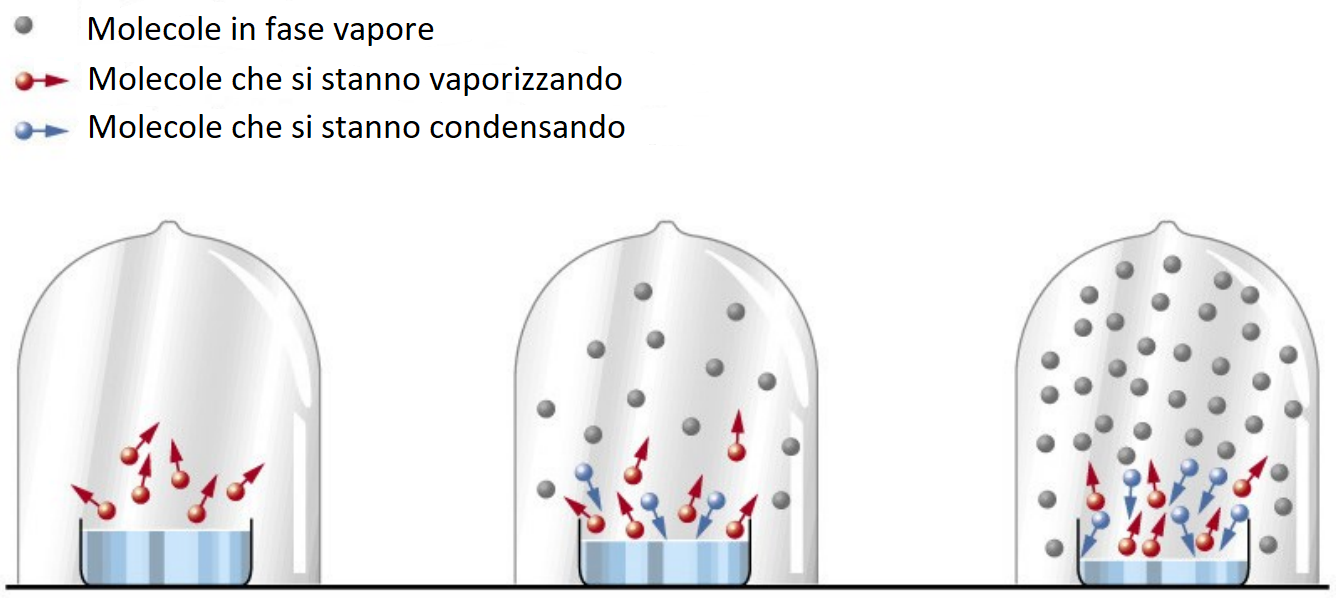
\includegraphics[width=15cm]{immagini/campana_di_vetro}
\end{figure}

Sarà opportuno racchiudere il contenitore con una campana di vetro in cui è preventivamente fatto il vuoto in modo da non avere particelle diverse da quelle del liquido.

Si lascia poi evaporare, o meglio si attende fino a quando si stabilisce un equilibrio, in quanto alcune particelle del liquido ne abbandonano la superficie per passare in fase vapore. Altre particelle nella fase vapore tenderanno invece a tornare nella fase liquida e ad un certo punto si raggiunge un equilibrio in cui la pressione delle particelle del liquido che sono passate dalla fase liquida a quella vapore è detta \textit{tensione di vapore} o pressione di vapore. Essa sarà la pressione esercitata sulle pareti della campana di vetro, in quanto avendo fatto il vuoto non ci sarà altra pressione.

Il fenomeno di passaggio da uno stato all'altro delle particelle dipende dalla temperatura, per cui a temperatura costante si avrà pressione costante dovuta solo alle particelle in fase vapore.

\vspace{0.2cm}\E chiaro che questo è un equilibrio dinamico: continuamente delle particelle che stanno in fase vapore tornernanno a far parte della fase liquida e viceversa dalla superficie del liquido altre particelle passeranno allo stato di vapore, ma nell'istante in cui si raggiunge tale equilibrio la tensione di vapore non cambia.

Inoltre il numero di particelle che abbandona la fase liquida per passare alla fase di vapore cresce all'aumentare della temperatura.

\hspace{0.5cm}\begin{minipage}{0.5 \textwidth}
    \begin{figure}[H]
        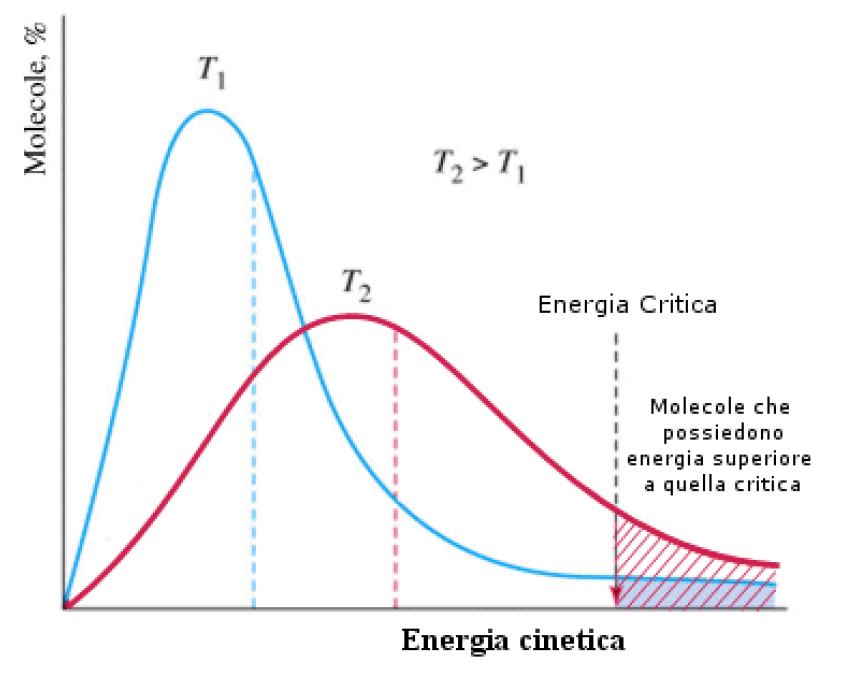
\includegraphics[width=7cm]{immagini/energie_fase_liquida.png}
    \end{figure}
\end{minipage}
\begin{minipage}{0.4 \textwidth}
\vspace{0.5cm}Dal grafico si evince che l'andamento a due diverse temperature mostra un picco nella percentuale di molecole che possiede una data energia e all'aumentare della temperatura tale picco si sposta a più alta energia e tende ad appiattirsi.
\end{minipage}

\vspace{0.2cm}Deduciamo che la percentuale di molecole ad alta energia è maggiore all'aumentare della temperatura, e siccome le particelle che riescono a passare dalla fase liquida a quella vapore sono quelle a più alta energia ne segue che aumenta il numero di quest'ultime.

\hspace{0.5cm}\begin{minipage}{0.5 \textwidth}
    \begin{figure}[H]
        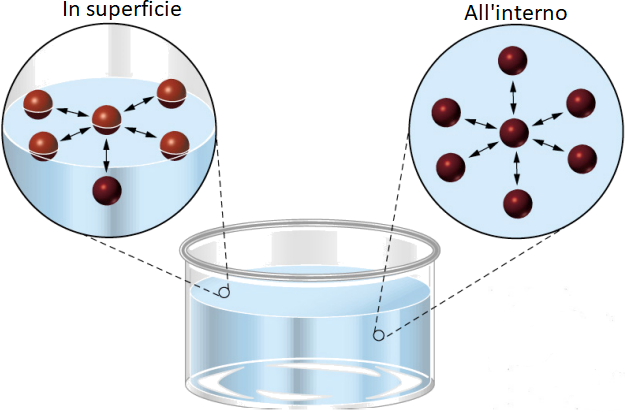
\includegraphics[width=7cm]{immagini/interazioni_nel_liquido.png}
    \end{figure}
\end{minipage}
\begin{minipage}{0.5 \textwidth}
    \begin{figure}[H]
        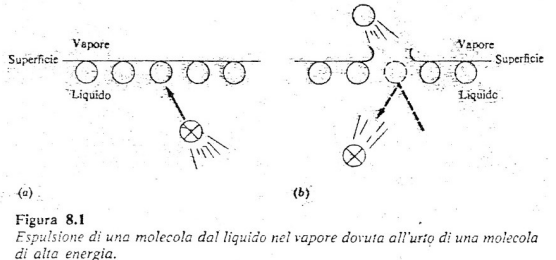
\includegraphics[width=7cm]{immagini/espulsione_particelle.png}
    \end{figure}
\end{minipage}

\vspace{0.4cm}Va da ricordare che all'interno del liquido qualunque particella è sottoposta a delle interazioni in tutte le direzioni. Viceversa sulla superficie del liquido la particella è sottoposta solo ad alcune di queste interazioni perché alcune mancano.

Si può dire che le particelle che passano da liquido a vapore vengano in qualche modo spinte dalle particelle interne con urti.

\subsection{La temperatura di ebollizione}
\vspace{0.2cm}Definiamo poi \textit{temperatura di ebollizione} per qualunque sostanza la temperatura alla quale la tensione di vapore di tale sostanza eguaglia la pressione atmosferica.

\hspace{0.5cm}\begin{minipage}{0.5 \textwidth}
    \begin{figure}[H]
        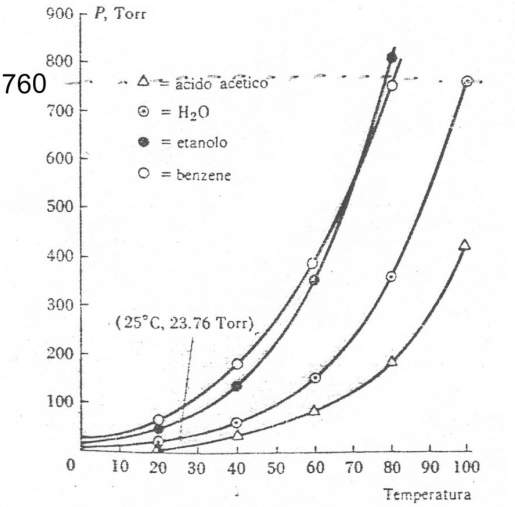
\includegraphics[width=6cm]{immagini/tensioni_di_vapore.png}
    \end{figure}
\end{minipage}
\begin{minipage}{0.4 \textwidth}
\vspace{0.5cm}Notiamo dal grafico che la tensione di vapore dei diversi composti, a parità di temperatura, è diversa.

\vspace{0.2cm}Ad esempio a parità di temperatura l'acqua mostra una tensione di vapore più bassa di quella dell'etanolo o del benzene, ma più alta dell'acido acetico.
\end{minipage}

\E importante quindi capire perché composti diversi mostrino tensioni di vapore diverse a parità di temperatura.

A naso si potrebbe dire che la massa delle particelle determinerà questa caratteristica, per cui particelle con massa maggiore eserciteranno, a parità di temperatura, una tensione di vapore minore rispetto quelle con massa minore, ma spesso non è così. Si vede anche nel grafico: il benzene C$_6$H$_6$ ha peso molecolare maggiore dell'acqua H$_2$O, ma a parità di temperatura ha tensione di vapore maggiore.

\begin{figure}[htp]
    \centering
    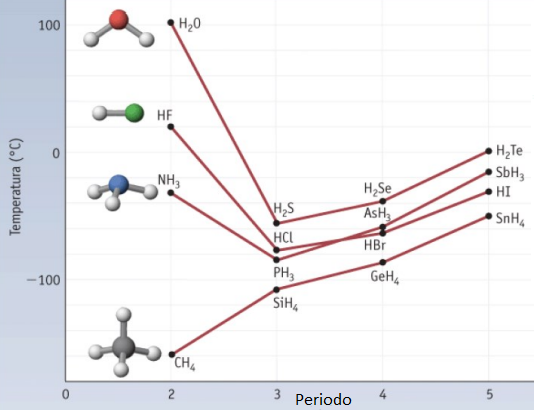
\includegraphics[width=12cm]{immagini/temperature_ebollizione.png}
\end{figure}

Consideriamo gli idruri del quarto gruppo: essi mostrano una temperatura di ebollizione che aumenta all'aumentare della massa.

Per tutti gli altri gruppi, se non consideriamo il primo composto l'andamento è ancora crescente. I capostipiti invece scartano molto dall'andamento della temperatura di ebollizione proporzionale alla massa. Se infatti li consideriamo, notiamo un netto crollo della temperatura di ebollizione all'aumentare della massa:

\begin{center}
    \begin{tabular}{m{2cm}m{2cm}m{2cm}m{2cm}}
    CH$_4$ & NH$_3$ & H$_2$O & HF\\[0.8ex]
    \hspace{-0.4cm}-161.5° C & \hspace{-0.3cm}-34.4° C & \hspace{-0.2cm}100° C & \hspace{-0.3cm}19.9° C\\[0.8ex]
    & PH$_3$ & H$_2$S & HCl\\[0.8ex]
    & \hspace{-0.3cm}-87.7° C & \hspace{-0.3cm}-60.3° C & \hspace{-0.3cm}-85.1° C\\[0.8ex]
    &&& HBr\\[0.8ex]
    &&& \hspace{-0.3cm}-66.7° C
    \end{tabular}
\end{center}

La seguente tabella mostra le temperature di ebollizione dei vari composti.

\vspace{0.2cm}C'è allora qualcos'altro oltre alla dipendenza dalla massa.

Questo qualcosa sono le interazioni intermolecolari presenti nei capostipiti di ogni gruppo, che si chiamano \textbf{legami a idrogeno}. Ne parleremo meglio in seguito.

\begin{minipage}{0.39 \textwidth}
    \begin{figure}[H]
        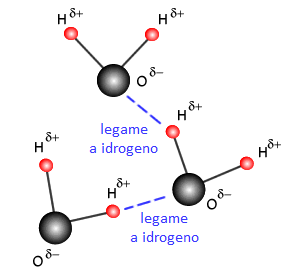
\includegraphics[width=6cm]{immagini/legame_a_idrogeno.png}
    \end{figure}
\end{minipage}
\begin{minipage}{0.6 \textwidth}
Esse sono presenti tra le molecole dell'acqua, e sono così forti (va da ricordare che per passare allo stato di vapore si devono rompere queste interazioni) da determinare un punto di ebollizione molto più elevato degli altri composti, in cui queste interazioni sono assenti pur avendo la stessa configurazione elettronica esterna.

Similmente ci sono delle interazioni che si esercitano tra le molecole di HF che siamo costretti a rompere se vogliamo portare l'acido fluoridrico allo stato di vapore, le quali sono presenti in maniera molto più contenuta nelle molecole HCl, HBr e HI.

Lo stesso dicesi per l'ammoniaca rispetto alla fosfina (PH$_3$), l'arsina (AsH$_3$) e la stibina (SbH$_3$).
\end{minipage}

\vspace{0.2cm}Quindi ci sono dei composti che in fase liquida esercitano delle interazioni intermolecolari fra le varie molecole che sono forti e che vanno rotte per ottenere vapore. Queste interazioni molto forti sono responsabili degli alti punti di ebollizione di queste molecole.